\chapter{Analysis of $\gamma$-ray from North and South Directions}
\label{appendix:ns_analysis}


According to photon intensity in Earth's centered coordinates
shows the higher density in the North-South direction comparing 
the East-West direction (Figure \ref{fig:flxmap_polar}).
The clue might come from exposure time in the North and South direction
is much higher than the east and west in Figure \ref{fig:expmap_polar}.
Performing an analysis of the North-South's $\gamma$-ray spectrum 
to compare with the full limb's photon could be a good option for 
investigating the quality of the analysis.

The North-South spectrum is obtained by applying condition of 
$\phi_\text{NADIR} \in (-30^{\circ}, 30^{\circ})$ for collecting
spectrum from the North and the $\phi_\text{NADIR} \in (150^{\circ}, 210^{\circ})$
for accumulating the spectrum from the South. The $\gamma$-ray
spectrum is plotted in Figure \ref{fig:ns_fit_gamma} on par with 
the optimization results from both SPL and BPL models.


\begin{figure}[h]
    \centering
    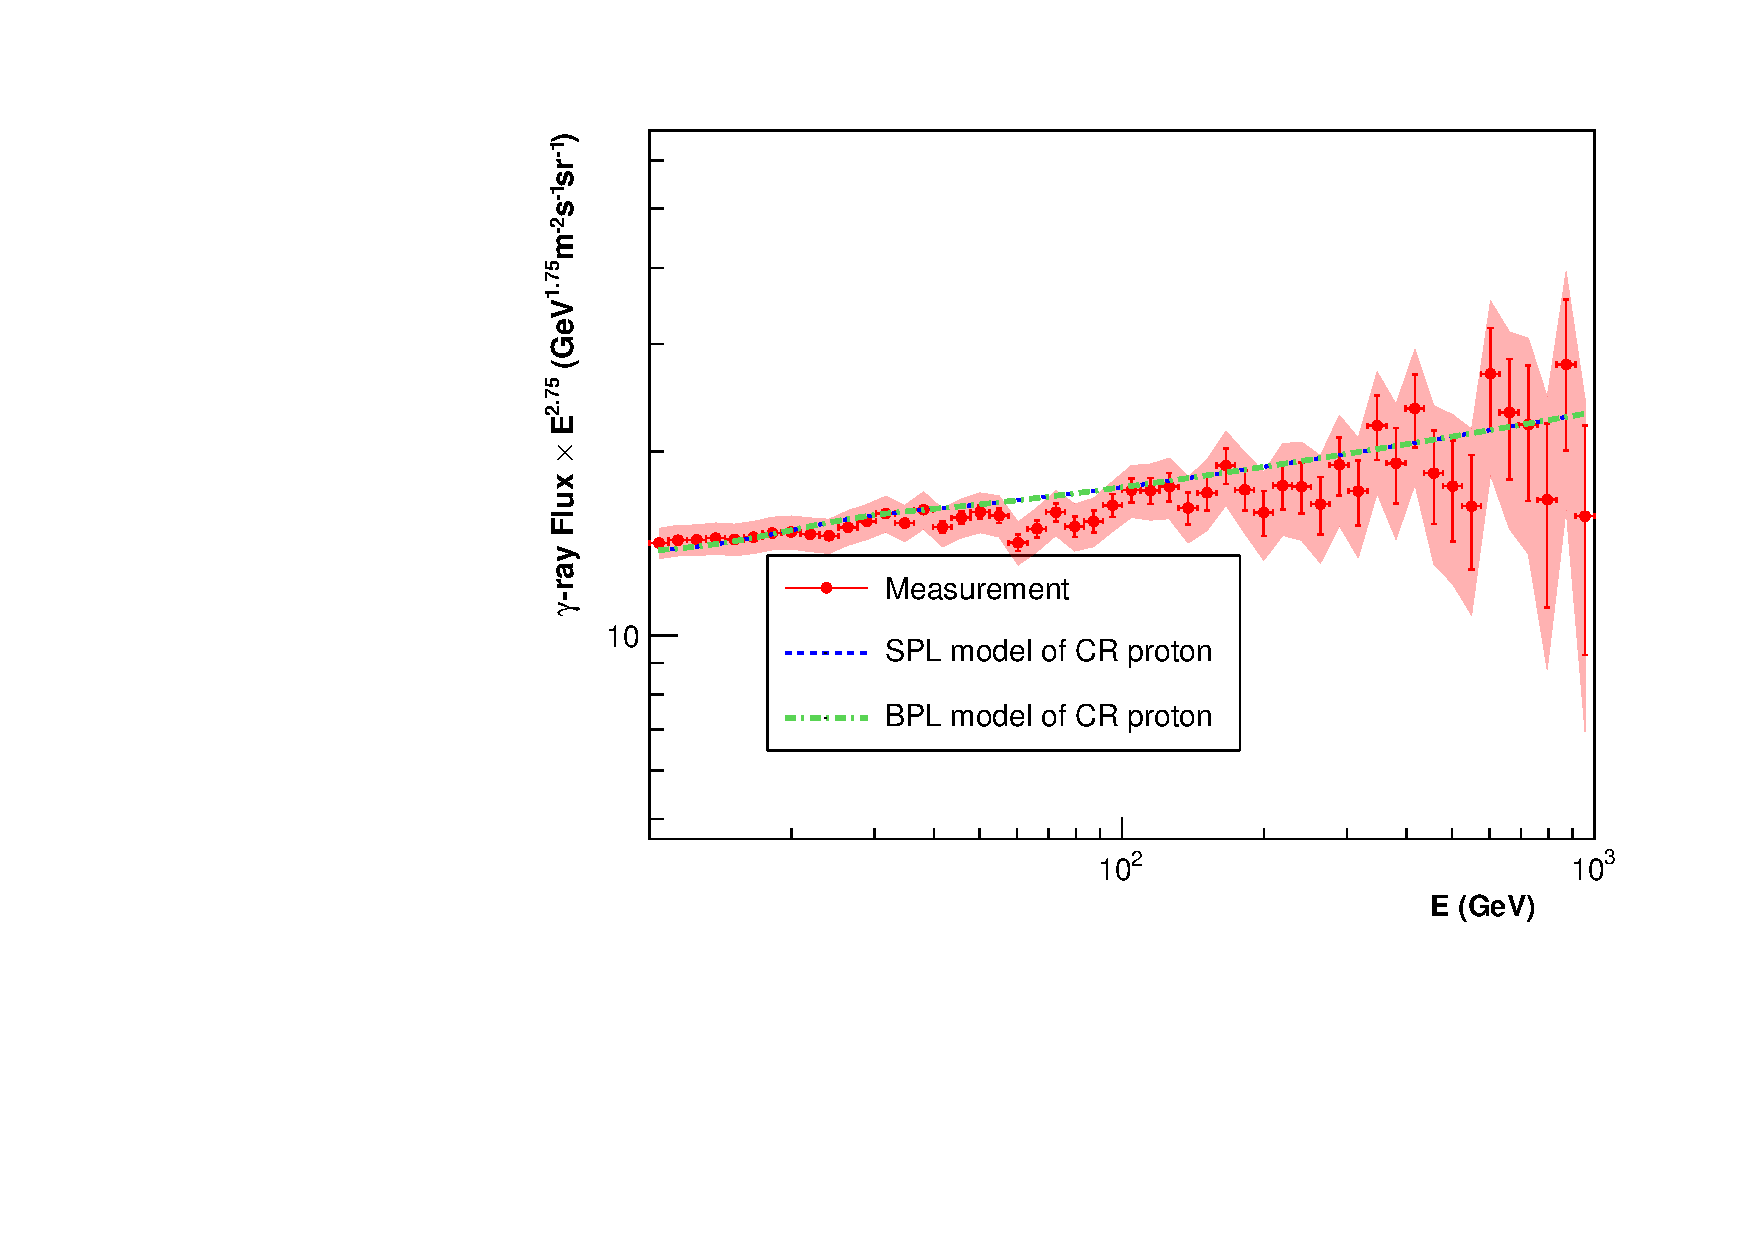
\includegraphics[width=0.8\textwidth]{appendix/ns_analysis/figures/fitted_result.pdf}
    \caption{North-South limb's $\gamma$-ray spectrum and the fitted models.}
    \label{fig:ns_fit_gamma}
\end{figure}

Table \ref{tb:bestfit_ns} shows the fitted parameters from
particle swarm optimization and the scaled results of modeled
proton spectrum is visualized in Figure \ref{fig:ns_vsother}.
According to Table \ref{tb:bestfit}, the outcome from this analysis 
shows the consistency where it aligns within 1$\sigma$ of the deviation.

\begin{table}[h!]
    \centering
    \begin{tabular}{l | c | c | c}
      Best fits & $\Gamma_1$ & $\Gamma_2$ & $E_{\text{Break}}$ (GeV) \\
      \hline \hline
      SPL & 2.63 & - & -  \\
      BPL & 2.90  & 2.65 & 327
    \end{tabular}
    \caption{Optimization results from the North-South spectrum.}
    \label{tb:bestfit_ns}
\end{table}

\begin{figure}[h]
    \centering
    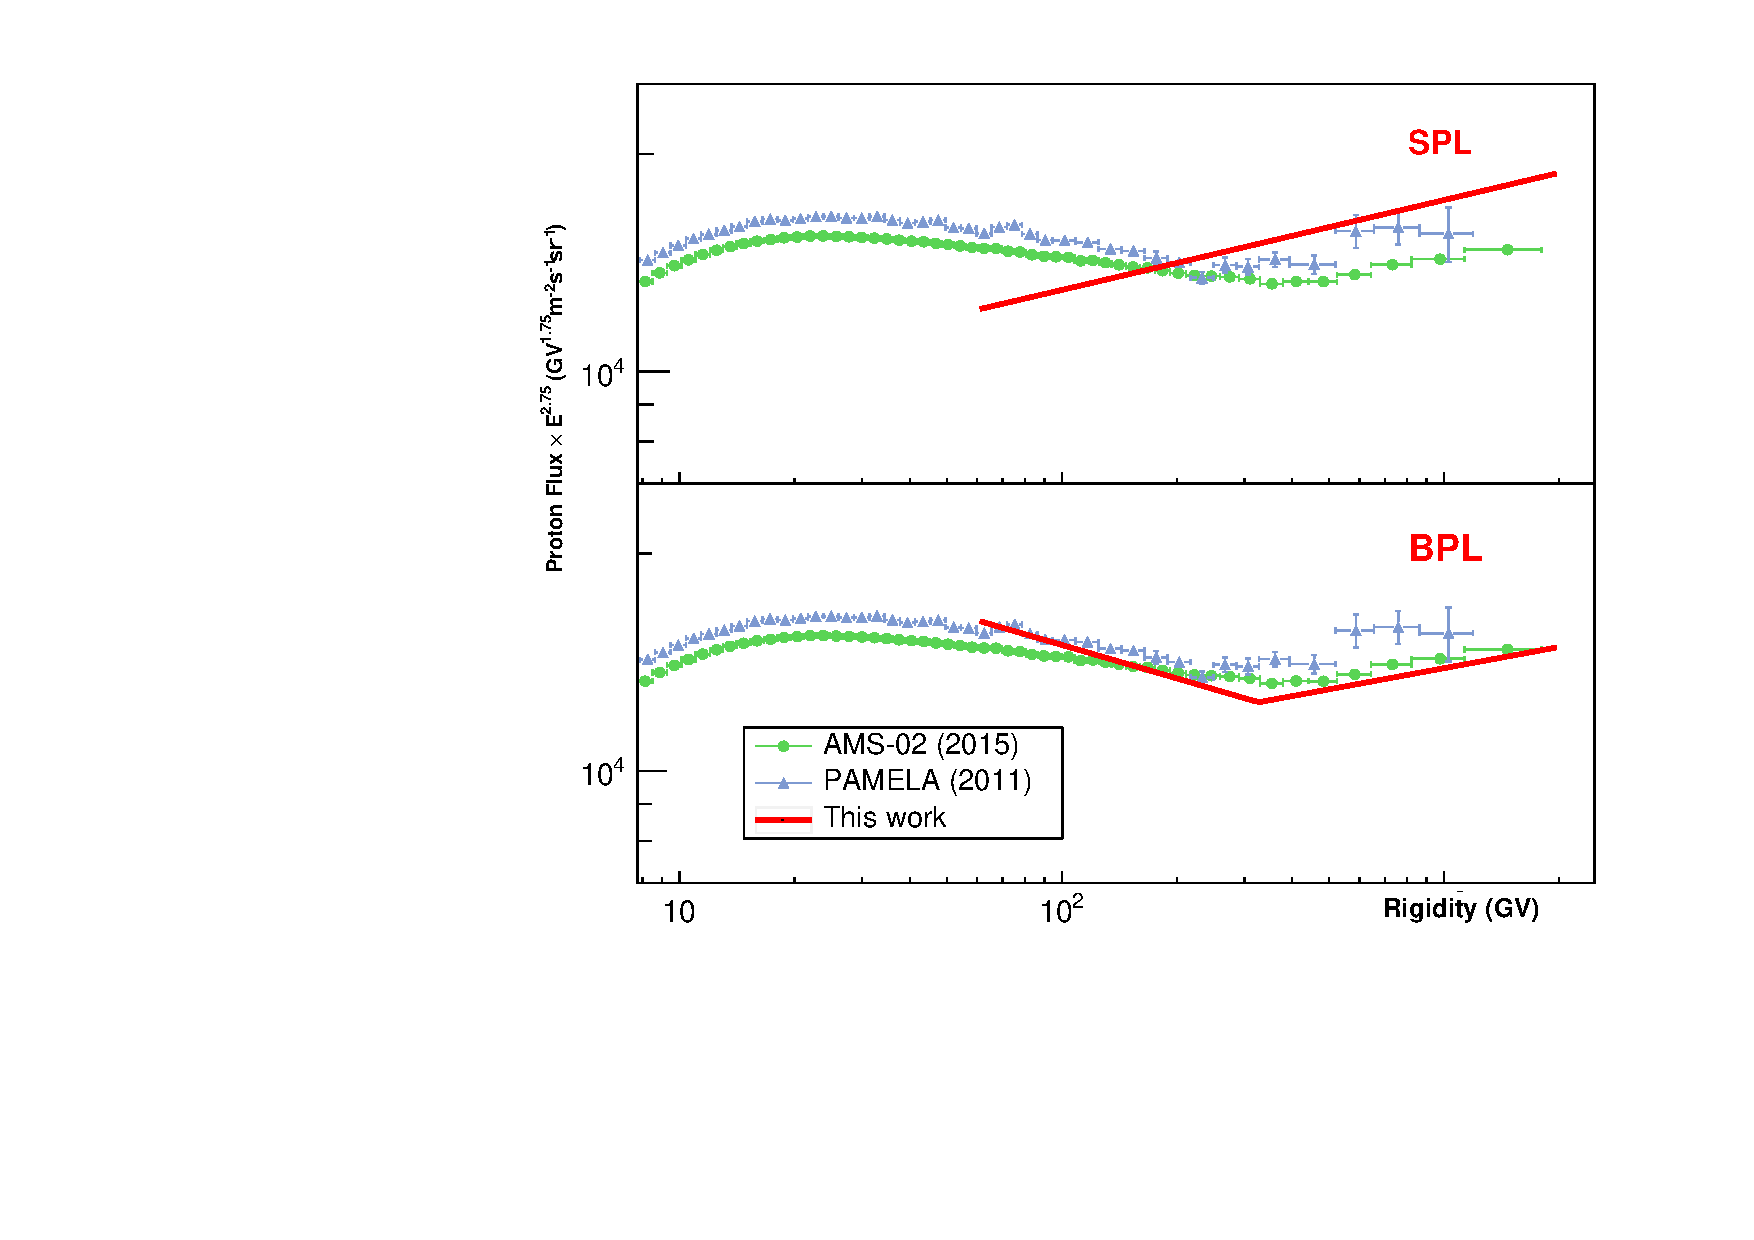
\includegraphics[width=0.9\textwidth]{appendix/ns_analysis/figures/vsother.pdf}
    \caption{
        Best-fit CR proton spectrum from 
        North-South $\gamma$-ray spectrum (red)
        compared to the measurements by
        AMS-02 (blue) and PAMELA (green).
    }
    \label{fig:ns_vsother}
\end{figure}

